\documentclass[14pt, a4paper]{article}

\usepackage{amssymb}
\usepackage{extsizes}
\usepackage{graphicx}
\usepackage{xcolor}
\usepackage{caption}
\usepackage{listings}
\usepackage{tabularx}
\usepackage{indentfirst}
\usepackage[T2A]{fontenc}
\usepackage[utf8]{inputenc}
\usepackage[english,russian]{babel}
\usepackage[left=30mm, right=10mm, top=20mm, bottom=20mm]{geometry}
\usepackage{ucs}

\graphicspath{{images/}}

\linespread{1.3}
\setcounter{tocdepth}{4}
\setlength{\parskip}{1.5pt}

\begin{document}
	\section{Семинар. UNIX}
	
	Процесс в UNIX - основная абстракция системы.
	Так во всех ОС [...]
	
	Поток - часть кода программы, которая может выполняться с другими частями кода программы. Именно потоком выделяется процессорное время.
	Когда выполняются потоки, они требуют ресурсы. Единицей диспетчеризации является поток. [посмотреть, что делает диспетчер]
	
	Диспетчеризация - выделение потока процессорного времени. Выделенные ресурсы принадлежат процессу.
	
	С точки зрения UNIX процесс часть времени выполняется в режиме пользователя (задачи), и тогда он выполняет собственный код, часть времени -
	в режиме ядра, и тогда он выполняет реентерабельный (???) код ОС.
	
	Реентерабельный код - код чистых процедур. Любая ОС должна иметь реентерабельные коды (искл. - DOS, связано с тем, что DOS - создавалась как однозадачная система, в результате все, что относилось к многозадачному, выкидывалось)
	
	Повторная входимость - несколько процессов могут вызвать одну и ту же функцию ОС, находясь в разных точках (???)
	
	Реентерабельность достигается засчет того, что в кодах функций нет данных. Функции работают с глобальными структурами ядра (хотя, так нельзя говорить)
	
	В UNIX любой процесс создается системным вызовом fork (<<развилка>>).
	
	[что-то про fork-бомбу, смотреть записи в тетради]
	
	[продолжение смотреть в тетради]
	
	\section{Группы}
	
	Процессы группы \underline{могут} получать одни и те же сигналы.
	
	Важнейшая группа - терминальная группа. Все процессы, запущенные на данном терминале, являются его потоками.
	Процесс, вызвавший fork, становится создателем (лидером) группы.
	
	Важнейщее событие в системе - завершение процесса (потому что родитель может проанализировать [что-то] у потомка).
	
	COW - решение разделения данных (об оптимизированном fork). Результат - во всех совр. ОС используется управление памятью страницами по запросу (виртуальная страничная память).
	
	COW позволяет разделять одно адресное пространство, т.е. предок и потомок разделяют одно адресное пространство (предка). [про права доступа - в тетради]
	
	О копировании: до тех пор, пока потомок не вызовет exit или exec (два сист. вызова; ОС не контролирует, в какой ветке вызываеются, потому что потомок - потенциальный родитель; это привело бы к слишком сложному анализу)
	
	Системный вызов exec переводит процесс на новое адресное пространство программы, которое передано exec в качестве параметра. Сначала exec проверяет, существует ли данный файл (речь идет о полном имени файла - состоит из пути к файла и имени файла; в UNIX/Linux начинается с /; эта строка символов проверяется до слеша, то есть программа проходит по каталогам, проверяя, существует ли файл или нет)
	
	Три типа файлов: исполняемые, объектные (obj) и исходные
	
	Нашла система файл. Далее проверка - исполняемый или нет. Если да, то проверяет, есть ли у процесса соответствующие права. Если все благополучно, то для программы, которая передана exec, создается адресное пространство, т.е. создаются карты трансляции адресов, которые в современных системах - таблицы страниц (в совр системах адресные пространства очень большие, для их описания нужно большое количество таблиц страниц).
	
	Доп.: В современных компах на базе процессоров Intel (64разр) схема преобразования называется PAE (???). Там 4 уровня таблиц.
	
	Дескриптор процесса имеет указатель на таблицы страниц. При создании новой таблицы указатель меняется (удалить -> поменять указатель -> в регистр CR3 (в Intel) загрузить адрес таблицы страниц из дескриптора -> в результате, будет выполняться новая программа). COW сбросится и установиться RW.
	
	\section{Если предок вызвал wait}
	
	[картинка]
	
	Если процесс блокирован, значит ему не выделяется процессорное время (для системы это плохо, потому что он занимает ресурсы).
	Поэтому вводится состояние zombie.
	
	zombie - это процесс, у которого отобраны все ресурсы, кроме последнего - строки таблицы процессов (такой таблицы нет; просто словосочетание, так было написано). Эта строка - дескриптор.
	
	Когда создается процесс, система сначала индентифицирует его (дает идентификатор) и выделяет ему структуру [скорее всего дескриптор] с большим количеством полей.
	
	\section{О pipe}
	
	pipe (<<труба>>) - потоковая модель передачи данных, симпликсная (односторонняя) связь
	
	pipe (программный канал) - [...]
	
	Системный вызов pipe создает неименованный программный канал
	
	Основной парадигмой UNIX является: в Unix все - файл => программный канал - специальный файл без имени (в системе имя файла не является идентификатора (идентификатор - номер inode'a - дескриптора файла (???))).
	
	pipe также наследует, как и fork (???). В результате через pipe могут взаимодействовать только процессы родственники.
	
	На самом деле pipe - это буфер в области данных ядра системы, потому что адресные пространства процессов являются защищенными. Это значит, что ни один процесс не может обратиться в адресное пространство другого процесса. Защита адресных пространств - основа многозадачности.
	
	Взаимодествовать параллельные процессы могут только через третье адресное пространство (системы). Это касается любого взаимодействия системы.
	
	[картинка]
	
	pipe был добавлен с механизмом взаимоисключения (???): в канал нельзя писать, если из него читают; нельзя читать, если пишут.
	
	В программных каналах присутствует файловый дескриптор (???)
	
	[код]
	
	Каналы в UNIX: именованные и неименованные
	
	\section{Об exec}
	
	execl(char *name, char arg0, ..., char argn, 0);
	
	execv(char *name, char *argv[]);
	
	execle(...) (???)
	
	excve(...) (???)
	
	\section{ЛР 2}
	
	Про ps:
	
	super user имеет доступ к функциям и структурам ядра
	
	Стэйты:
	
	D (device - любое внешнее устройство) - непрерываемый сон (обычно ввод/вывод). Это значит, что процесс, ожидающий завершения ввода/вывода, не может быть выведен из состояния блокировки (sleep). Блокированный процесс не получает процессорное время.
	
	S - сон, который
	
	R - {\bf система не различает}, выполняется ли процесс или ждет выполнения в {\bf очереди готовых процессов}
	
	\section{Системные демоны}
	
	1 - [...]
	2 - [...]
	
	Все kill к системным демонам игнорируются.
	
	Демоны ПРЦПУ(???) на процессор (со слешами).
	
	\section{ls}
	
	d – справочник или директорий (directory)
	
	-  - обычный файл (regular)
	
	l – символическая связь (канал) – символьная ссылка
	
	b – специальный блочный файл - блочное устройство (block device)
	
	c – специальный символьный файл - символьное устройство (character)
	
	p – программный канал (pipe) (именованный)
	
	s – сокет в файловом пространстве имен (Домен – UNIX)
	
	Короткая формула:
	
	hard link - еще одно полноправное имя файла. В UNIX имя файла не является его идентификатора.
	
	soft link - [...]
	
	\pagebreak
	
	\section{Лекция 3}
	\subsection{Планирование и диспетчеризация}
	
	Планирование (sheduling) - определение очередности выполнения работы (в общем-то).
	
	Планировщик ставит процессы в очередь по каким-то критериям.
	
	Диспетчеризация - непосредственно выделение процессу процессорного времени.
	
	В зависимости от типа ОС это делается по разному: учитываются особенности ОС.
	
	\subsection{Алгоритмы планирования}
	
	1. Алгоритмы планирования в системах пакетной обработки (дисциплины планирования).
	
	1.1 FIFO (First In First Out) (или FCTS - First Come First)
	
	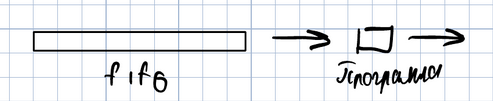
\includegraphics[width=\linewidth]{1}
	
	Мы будем рассматривать алгоритмы с точки зрения того, как выполняется программа (от начала до конца, или ее выполнение может быть прервано).
	
	Что касается FIFO, то в данном случае - простая очередь, и программа выполняется от начала до конца. Все задания равноправны, т.е. нет приоритетов.
	
	1.2 SYF (Sortest Job First) (наикротчайшее задание первым)
	
	Предпочтение отдается коротким заданиям (заданиям, требующим малое количество времени на выполнение).
	
	Зачем так сделали? Система mainframe - дорогая. Ее эффективная работа является приоритетной задачи. Как оценить эффективность? Как количество заданий, выполненных за единицу времени.
	
	Однако эта система планирования привела к негативному эффекту - <<бесконечное откладывание>>: поступают короткие задания, они ставятся в очереди вперед других, в итоге задания, требующие большее количество времени, могут просто не выполниться.
	
	Доп. Программы можно было <<пустить вперед>>.
	
	1.3 SRT (Shortest Remaining Time) (динамический пересчет приоритетов)
	
	Предполагает, что выполняющееся задание может быть прервано, если поступит задание с меньшим оценочным временем выполнения.
	
	Процесс с большим оценочным временем вытесняется процессом с меньшим оценочным временем.
	
	Для реализации система должна отслеживать время выполнения.
	
	Та же проблема с бесконечным откладыванием.
	
	А что делать с вытесненными процессами? Чтобы иметь возможность продолжить выполнение процесса (не с начала), необходимо сохранить аппаратный контекст.
	
	1.4 HRN (Highest Response Ratio Next) (динамический пересчет приоритетов)
	
	Появился как ответ на проблему бесконечного откладывания.
	
	Приоритет вычисляется по формуле: $$p = \frac{t_w + t_s}{t_s},$$
	
	где $t_s$ - запрошенное время выполнения, $t_w$ - время ожидания (простоя) в очереди готовых процессов. Чем больше время ожидания, тем выше приоритет. То есть с течением времени процесс получит процесорное время.
	
	? Найти, каким образом в винде и Unix учитывается приоритет процессов (в книгах Русиновича и Вахалия).
	
	2. Системы разделения времени (sharing time)
	
	Суть - появление возможности интерактивного взаимодействия пользователя с программой.
	
	!!! DOS таковым не является
	
	2.1 RR (Round Robin) - алгоритм циклического планирования.
	
	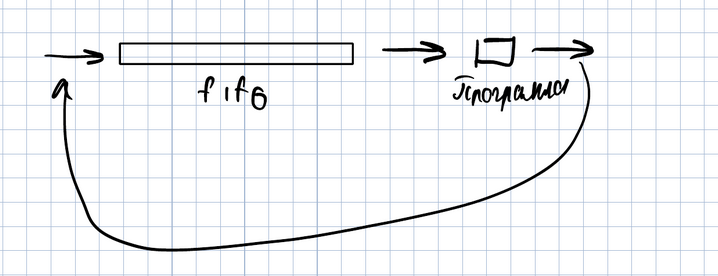
\includegraphics[width=\linewidth]{2}
	
	Процессу выделяется квант. Исчерпава его, процесс возвращается в хвост очереди.
	
	2.2 Адаптивное планирование (или многоуровневые очереди)
	
	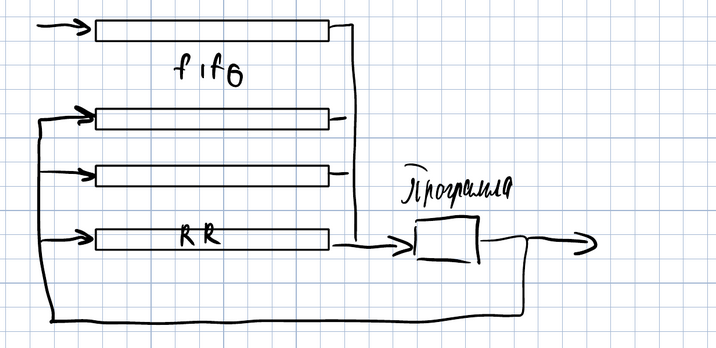
\includegraphics[width=\linewidth]{3}
	
	Предполагают, что существует несколько очередей (FIFO). Каждая очередь работает по RR и имеет свой приоритет.
	
	В первую очередь поступают только что созданные процессы и процессы, завершившие ожидание ввода/вывода.
	
	! Следует подчеркнуть, что <<процесс блокирован>> означает, что процесс не получает процессорного времени.
	
	Если процесс за выделенный квант не успел завершиться или выдать запрос на ввод/вывод, он перемещается в следующуюю менее приоритетную очередь, пока не окажется в очереди RR (в котором крутится т.н. {\bf холостой процесс}).
	
	Какие задания оказываются в последней низкоприоритетной очереди (для чего нужно много процессорного времени):
	
	- вычислительные процессы
	
	Алгоритм учитывает (неявно) процессорное время (не только время простоя, но и получения процессорного времени)
	
	\subsection{Вернемся к диаграмме состояния процесса}
	
	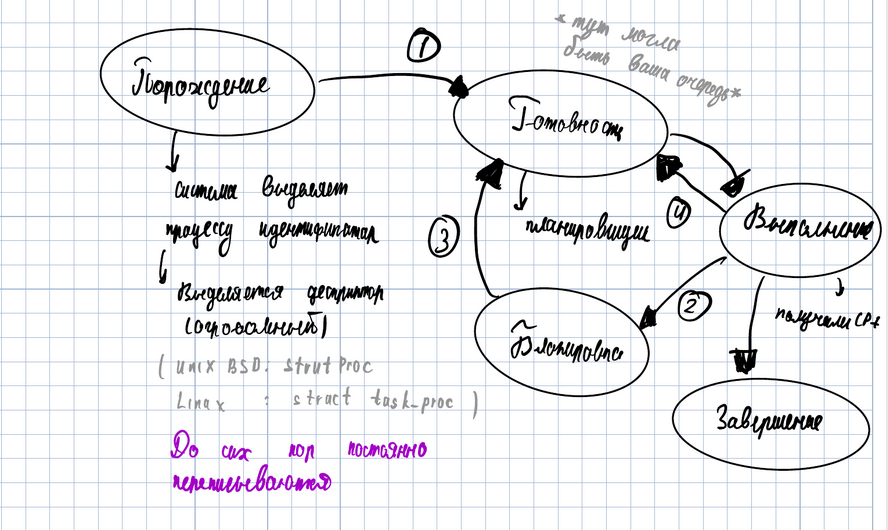
\includegraphics[width=\linewidth]{4}
	
	Первое, что делает система, - порождение процесса (выделение процессором идентификатора -> процессору выделяется дескриптор - огромная структура -> [создается адресное пространство] -> выделить физическую память (???) -> процесс переходит в состояние готовности).
	
	В состоянии готовности находится очень много процессов -> очередь [написать про планировщик]
	
	Из состояния готовности - в состояние выполнения (процесс получает процессорное время)
	
	Из состояния выполнения - в состояние завершения
	
	В системе, в котором реализован принцип распараллеливания функций, перейти в режим блокировки (из выполнения).
	
	Блокировка возможна, когда процесс запросил дополнительный ресурс.
	
	Из блокировки - в состояние готовности (получил доп ресурсы - может продолжить)
	
	\section{Классификация алгоритмов планирования}
	
	1.
	
	- с переключением
	
	- без переключения
	
	2.
	
	- с приоритетами
	
	- без приоритетов
	
	3. (следует из 2.)
	
	- с вытеснением
	
	- без вытеснения
	
	Приоритеты бывают статическими (назначаются процессом до начала выполнения и не меняются) и динамическими (назначаются при выполнении); абсолютные (назначаются из какой-то шкалы) и относительные (по какому-то приоритету (???))
	
	{\bf Опр.} Sheduling algorithm - алгоритм, используемый для определения того из нескольких процессов, с одинаковой степенью пригодных для распределения им ресурса, которому этот ресурс будет предоставлен.
	
	В очереди могут находится процессы, получившие все ресурсы, кроме процессорного времени.
	
	\section{Потоки (thread)}
	
	Поток имеет две характерные черты:
	
	1. Владение ресурсами (ownership): адресное пространство, которое содержит образ процесса (владеет все время существование процесса)
	
	2. Планирование и выполнение (sheduling and execution). Для этого нужно процессорное время, при этом время выполнения чередуется с временем простоя (ожидания).
	
	Вторая характеристика может быть отделена от процесса и передана его части.
	
	{\bf Опр.} Поток - это часть кода программы, которая может выполняться параллельно с другими частями кода.
	
	{\bf Поток не имеет собственного адресного пространства и выполняется в адресном пространстве процесса.}
	
	Поток владеет аппаратным контекстом. При этом получается, что не процессу выделяется процессорное время, а потоку -> единицей диспетчеризации становится поток. В результате командой за командой выполняется часть кода программы, переданной потоку (???). Поток может запрашивать ресурсы, но их владельцем остается процесс.
	
	При этом надо все сводить к общности. Если в программе дополнительные потоки не создаются, то считаеся, что в программе выполняется один главный поток.
	
	Таким образом, в современных системах потоки являются базовой единицей выполнения процесса.
	
	Поток владеет счетчиком команд, стеком, набором регистров (аппаратный контекст), идентификатором thread\_id.
	
	Коль программа может иметь несколько потоков (или не иметь их), имеются две модели: однопоточный и многопоточный.
	
	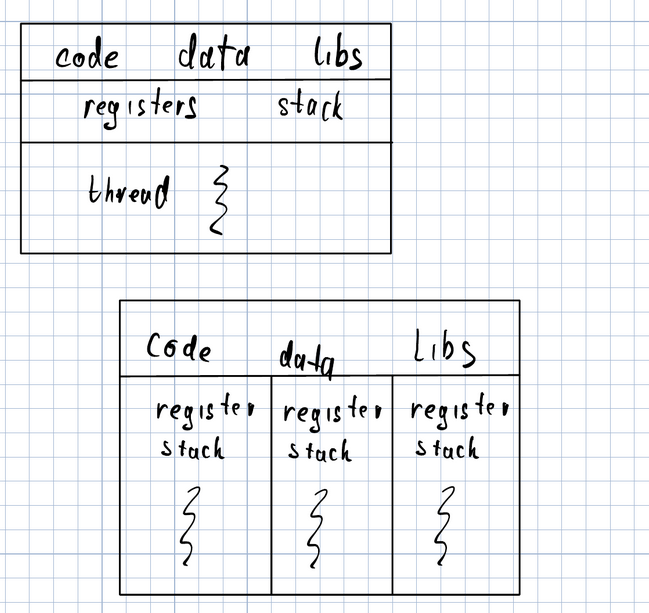
\includegraphics[width=\linewidth]{5}
\end{document}
